\documentclass{article}


\usepackage{style}

\usepackage[utf8]{inputenc} % allow utf-8 input
\usepackage[T1]{fontenc}    % use 8-bit T1 fonts
\usepackage{hyperref}       % hyperlinks
\usepackage{url}            % simple URL typesetting
\usepackage{booktabs}       % professional-quality tables
\usepackage{amsfonts}       % blackboard math symbols
\usepackage{nicefrac}       % compact symbols for 1/2, etc.
\usepackage{microtype}      % microtypography
\usepackage{fancyhdr}       % header
\usepackage{graphicx}       % graphics
\graphicspath{{media/}}     % organize your images and other figures under media/ folder
\usepackage{longtable,booktabs,array}
\usepackage{calc} % for calculating minipage widths


%Header
\pagestyle{fancy}
\thispagestyle{empty}
\rhead{ \textit{ }} 

% Update your Headers here
\fancyhead[LO]{GAT - Attention and Memory}
% \fancyhead[RE]{Firstauthor and Secondauthor} % Firstauthor et al. if more than 2 - must use \documentclass[twoside]{article}



  
%% Title
\title{GAT - Attention and Memory
}

\author{
  Annisa Haycal \\
  Bina Nusantara University \\
  \texttt{haycal.annisa@binus.ac.id} \\
  %% examples of more authors
   \And
  Catherine Benedicta \\
  Bina Nusantara University \\
  \texttt{benedicta.catherine@binus.ac.id} \\
  \And
  Sekar Azalea \\
  Bina Nusantara University \\
  \texttt{mardiah.sekar@binus.ac.id}
}


\begin{document}
\maketitle


\begin{abstract}
Model Graph Neural Network (GNNs) terkenal dengan penggunaannya untuk permasalahan suatu grafik. Dengan menerapkan mekanisme attention untuk menyelesaikan tugas ini, maka digunakanlah arsitektur Graph Attention Network (GATs) karena arsiterktur ini dianggap lebih akurat untuk permasalahan ini dibandingkan model GNN lainnya, karena mekanisme attention dapat menyelesaikan input node dengan ukuran yang berbeda-beda, dan hanya berfokus pada bagian yang penting. Dugaan ini dibuktikan dengan hasil eksperimen kami dengan membandingkan model GAT dengan model GCN. Dengan menggunakan dataset CORA, hasil akurasi yang didapatkan GAT lebih tinggi dibandingkan dengan hasil GCN.
\end{abstract}


% keywords can be removed
\keywords{attention, GAT, node classification}


\section{Introduction}
Permasalahan \textit{node classification} merupakan tugas dimana algoritma melakukan pengenalan mengenai label dari node-node tetangganya. Tugas ini memprediksi atribut dari setiap node dalam grafik. Misalnya, memberi label pada setiap node dengan kelas kategori (klasifikasi biner atau klasifikasi multi kelas), atau memprediksi angka kontinu (regresi). Tugas ini juga dilakukan untuk memprediksi node yang tidak ada, yang dapat dikenali berdasarkan properti node lainnya.

Model seperti Convolutional Neural Networks (CNNs) dan Recurrent Neural Networks (RNNs) umumnya dapat menyelesaikan permasalahan seperti \textit{node classification}. Namun, tantangan pada pendekatan ini adalah dimana algoritma harus menentukan operator yang bekerja dengan node tetangga dengan properti yang berbeda. Pada beberapa kasus, hal ini membutuhkan pembelajaran mesin mengenai \textit{matrix weight} pada masing-masing node.

Mekanisme Attention telah menjadi suatu standar de facto pada beberapa masalah dengan \textit{many sequence-based}. Dan salah satu kelebihan dari menggunakan mekanisme adalah algoritma ini dapat menyelesaikan input node dengan ukuran yang berbeda-beda, dan hanya berfokus pada bagian yang penting. Dibandingkan dengan model CNNs dan RNNs, mekanisme ini sudah terbukti lebih berguna untuk masalah seperti machine reading. Tidak hanya itu, pada penelitian yang dilakukan Vaswani\cite{cite1} pada tahun 2017 menunjukkan bahwa mekanisme juga cukup untuk membangun model terbaik yang memperoleh kinerja canggih dalam tugas machine translation.

Berdasarkan penelitian ini, kita gunakan arsitektur berdasar mekanisme Attention untuk menyelesaikan tugas \textit{node classification} dari grafik terstruktur. Intinya adalah untuk menghitung representasi tersembunyi dari setiap node dalam grafik, dengan memperhatikan tetangganya. Arsitektur ini disebut dengan Graph Attention Networks atau GATs. Berdasarkan kutipan yang diambil dari beberapa artikel mengenai GATs, arsitektur ini merupakan salah satu arsitektur dari model GNNs (Zhang\cite{article2}). Maka dari itu, konsep dari arsitektur ini hampir sama dengan arsitektur buatan GNNs lainnya, yaitu GCNs (Labonne\cite{article3}).

\section{Previous Research}
Permasalahan \textit{node classification} sudah umum dilakukan. Permasalahan ini dapat diselesaikan dengan banyak cara dengan banyak model juga. Model CNNs dapat digunakan untuk menyelesaikan permasalahan \textit{node classification}. Walaupun pada dasarnya model ini bukan diperuntukkan untuk masalah grafik seperti yang ada di \textit{node classification}, namun dengan menggeneralisasikan model ini kepada grafik akan bisa memberikan kemungkinan untuk mencapainya. Penelitian yang pernah dilakukan sebelumnya pada tahun 2015 oleh Duvenaud\cite{cite4} dan lainnya membuat model CNNs yang beroperasi secara langsung terhadap grafik. Lalu, terdapat juga penelitian Atwood dan Tosley\cite{cite5} dan Hamilton\cite{cite6} yang mengambil konsep sama, yaitu untuk mengoperasikan model CNNs ke suatu grafik. Selain itu, penelitian yang dilakukan oleh Monti\cite{cite7} dan lainnya dengan membuat suatu model campuran CNN dengan nama MoNet juga dilakukan untuk mengoperasikan model CNN ke dalam grafik. 

Namun, keempat penelitian tersebut memberikan hasil kesimpulan bahwa untuk mengoperasikan model CNNs ke suatu grafik masih harus membutuhkan beberapa syarat tambahan. 

Berhubungan dengan model yang akan kami buat, penelitian yang telah dilakukan Santoro\cite{cite8} dan Schlichtkrull\cite{cite9} memiliki pendekatan yang hampir sama dengan kami, dimana pada penelitian ini membahas mengenai \textit{relational networks} akan berbagi informasi antar-node nya. Penelitian kami juga memiliki kesamaan konsep model \textit{attention} dengan penelitian yang dilakukan Duan\cite{cite10} dan Denil\cite{cite11} dimana memanfaatkan mekanisme attention di sekeliling node untuk menghitung koefisien attention antara node atau objek di lingkungannya.

Pendekatan yang sama juga pernah dilakukan pada penelitian yang dilakukan oleh Roweis dan Raul\cite{cite12} yang membuat model LLE (Locally Linear Embedding) dan Weston\cite{cite13} yang mengangkat topik mengenai memory networks. Model LLE akan menggunakan angka pasti dari tiap node tetangga dan mengumpulkan properti node-node tersebut, seperti koefisien bobot dari tiap nodenya. Dan dengan \textit{memory networks} menganggap tiap node di lingkungan sebagai sebuah memori yang menyimpan properti atau nilai. Dengan inilah kita bisa menghitung fitur-fiturnya dengan memperhatikan nilainya, dan kemudian informasi tersebut akan diperbarui dengan menyimpan fitur baru pada lokasi node yang sama.

Model dari metode GNNs atau Graph Neural Network yang bernama DEMO-Net juga pernah dilakukan oleh Wu\cite{cite14}. Pada penelitian ini, diusulkan konsep Multi-task Graph Convolution dimana tiap node akan direpresentasikan dengan tingkat yang berbeda-beda. Konsep ini tentunya sama dengan konsep \textit{attention} yang akan kita gunakan. Masih menggunakan metode GNN yang sama, penelitian yang pernah dilakukan oleh Fey\cite{cite15} dan Maurya\cite{cite16} meneliti untuk menyeleksi node yang akan dipakai. Berhubungan dengan kedua penelitian tersebut, Maurya\cite{cite17} juga meneliti bahwa berdasarkan properti yang dimiliki setiap node, peran yang akan dimainkan juga akan berbeda. Dengan mengetahui properti dari tiap node, akan membuahkan hasil yang kemungkinan dapat meningkatkan hasil dari eksperimen. Kipf\cite{cite18} juga meneliti sebuah representasi yang tersembunyi dari sebuah fitur node. Sebelumnya juga terdapat penelitian oleh Hussain\cite{cite19} yang mengangkat topik \textit{self-attention} pada GNNs dimana mekanisme \textit{attention} digunakan untuk melihat apakah terdapat interaksi antar-node pada lingkungannya saja (\textit{local self-attention}) atau seluruh input pada grafik (\textit{global self-attention}).

Terinspirasi dari penelitian-penelitian tersebut, penelitian kali ini mengangkat topik mekanisme \textit{attention} dengan arsitektur GAT atau Graph Attention Network. Penelitian yang pernah dilakukan sebelumnya yang juga menggunakan konsep seperti ini terbagi menjadi dua jenis pembelajaran, yaitu \textit{transductive} dan \textit{inductive}. Jenis \textit{transductive} pernah dilakukan oleh Sen\cite{cite20} dan Yang\cite{cite21}, sedangkan jenis \textit{inductive} dilakukan oleh Zitnik\cite{cite22}, Hamilton\cite{cite6}, dan  Subramanian\cite{cite23}.

Beberapa perbedaan penelitian yang pernah dilakukan dengan penelitian yang dilakukan pada paper ini dijelaskan secara singkat pada:

\begin{center}
\begin{tabular}{m{3cm}|m{3cm}|m{3cm}|m{3cm}|m{3cm}}
\hline
\textbf{Judul} & \textbf{Peneliti} & \textbf{Metode} & \textbf{Hasil} & \textbf{Perbedaan} \\
\hline
\textbf{Semi-Supervised Classification With Graph Convolutional Networks\cite{cite18}} & \textbf{Thomas N. Kipf dan Max Welling} & \textbf{Mereka membuat struktur grafik menggunakan model \textit{neural network} dan men-\textit{train supervised target} untuk semua node dengan label. Penyelesaian masalah dengan berdasarkan metode GCN.
} & \textbf{Model GCN yang diusulkan berhasil untuk meng-\textit{encode} struktur grafik dengan fitur node yang berguna untuk usahanya dalam percobaan \textit{semi-supervised classification}} & \textbf{Metode yang digunakan masih membutuhkan beberapa ketentuan, seperti eigendecompositions dan operasi matriks tentang bobot dari node. Model kami secara implisit memungkinkan untuk langsung menentukan mana node yang lebih penting untuk dikunjungi.} \\ 
\hline 
\end{tabular}
\end{center}

\begin{center}
\begin{tabular}{m{3cm}|m{3cm}|m{3cm}|m{3cm}|m{3cm}}
\hline
\textbf{Watch Your Step: Learning Node Embeddings via Graph Attention\cite{cite24}} & \textbf{Sami Abu-El-Haija, Bryan Perozzi, Rami Al-Rfou, Alex Alemi} & \textbf{Dalam makalah ini, mereka mengganti \textit{hyperparameter} dengan yang dapat dilatih yang secara otomatis berdasarkan \textit{backpropagation}} & \textbf{Akurasi yang dihasilkan pada model paper ini sebesar 67.9} & \textbf{Model GAT pada paper ini menggunakan \textit{hyperparameter} lain selain yang digunakan pada model GAT kita} \\
\hline
\textbf{Inductive Representation Learning on Large Graphs\cite{cite6}} & \textbf{William L. Hamilton, Rex Ying, Jure Leskovec} & \textbf{Paper ini  menyajikan model GraphSAGE, yang mana model ini merupakan kerangka kerja induktif umum yang memanfaatkan informasi fitur node untuk menghasilkan \textit{node embedding} secara efisien untuk data yang sebelumnya tidak terlihat} & \textbf{Pada model LSTM dari GraphSage (GraphSage-LSTM) menghasilkan akurasi 0.612} & \textbf{Implementasi dari GraphSAGE dan model GAT kita sangat berbeda, GraphSAGE berbasis sampel, di mana tetangga dari sebuah node dijadikan sampel sebagai nomor tetap, sementara GAT mempertimbangkan semua tetangga} \\
\hline
\textbf{Representation Learning on Graphs with Jumping Knowledge Networks\cite{cite25}} & \textbf{Keyulu Xu, Chengtao Li, Yonglong Tian, Tomohiro Sonobe} & \textbf{Metode yang digunakan pada paper ini adalah membuat skema agregasi baru untuk pembelajaran representasi node yang dapat mengadaptasi rentang lingkungan ke node secara individual. JKNet ini dapat meningkatkan representasi khususnya untuk grafik yang memiliki subgraf dengan struktur lokal yang beragam, dan karenanya mungkin tidak ditangkap dengan baik oleh agregasi lingkungan dalam jumlah tetap} & \textbf{Kesimpulan dari hasil penelitian yang dilakukan pada paper ini adalah bahwa model JKNets ini dapat meningkatkan representasi khususnya untuk grafik yang memiliki subgraf dengan struktur lokal yang beragam, dan karenanya mungkin tidak ditangkap dengan baik oleh agregasi lingkungan dalam jumlah tetap} & \textbf{Model yang kita pakai, yaitu GAT mencapai akurasi terbaiknya hanya dengan 2 atau 3 \textit{layer}, menunjukkan bahwa informasi lokal merupakan sinyal yang lebih kuat untuk klasifikasi daripada informasi global. Namun, JKNet mencapai akurasi terbaiknya dengan 6 \textit{layer} menunjukkan bahwa informasi global bersama dengan lokal akan membantu meningkatkan kinerja} \\
\hline
\textbf{Revisiting Semi-Supervised Learning with Graph Embeddings\cite{cite21}} & \textbf{Zhilin Yang, William W. Cohen, Ruslan Salakhutdinov} & \textbf{Paper ini menggunakan model bernama Planetoid. Metode yang dipakai yaitu melatih (\textit{train}) \textit{node embedding} di tiap instansi  untuk bersama-sama memprediksi label kelas dan konteks lingkungan dalam grafik} & \textbf{Angka akurasi yang dihasilkan dengan metode ini adalah 75.7} & \textbf{Model Planetoid pada paper ini yang digunakan merupakan penggabungan (\textit{embedding}) grafik untuk mengenali properti atau kelas label dari \textit{node neighbor}, sedangkan model GAT menetapkan angka weight yang berbeda di tiap \textit{neighborhood}} \\ \hline
\end{tabular}
\end{center}

\section{Methodology or Architecture Deep Learning}
\subsection{Node Classification}
Node Classification atau klasifikasi node adalah sebuah tugas machine learning umum yang diterapkan pada suatu grafik, dimana kita akan men-\textit{train} suatu model untuk mengklasifikasi node. Algoritma akan melakukan pengenalan mengenai label dari suatu node dan tetangganya. 
Tugas ini dilakukan untuk memprediksi atribut atau properti dari setiap node dalam grafik. Misalnya, \textit{node classification} dilakukan dengan memberi label pada setiap node dengan kelas kategori (klasifikasi biner atau klasifikasi multi kelas), atau memprediksi angka kontinu (regresi). Tugas ini juga dilakukan untuk memprediksi node yang tidak ada, yang dapat dikenali berdasarkan properti node lainnya.

\subsection{Graph Neural Networks}
GNN atau \textit{graph neural network} sendiri merupakan salah satu arsitektur deep learning yang digunakan untuk menyelesaikan masalah-masalah machine learning pada data yang berbentuk grafik. GNN ini dapat ditinjau sebagai bentuk umum dari Convolutional Neural Network (CNN) dari struktur kisi (piksel dalam gambar) yang cenderung ‘kaku’ menjadi data yang lebih fleksibel namun tetap terstruktur.

Data pada GNN, jelasnya, berbentuk vektor bilangan riil dengan alur pertukaran informasi yang tidak memiliki aturan ataupun giliran secara spesifik. Vektor awal kemudian mengalami agregasi setelah menerima data dari titik terdekatnya. Setelah adanya proses agregasi, perlu diputuskan hal apa yang ingin dikomputasikan. Terdapat dua pilihan pada GNN, yakni untuk mengkomputasi \textit{node-level function} atau \textit{graph-level function}. GNN sendiri memiliki jumlah layer atau lapis yang telah ditentukan, dengan setiap layer-nya memiliki fungsi agregasi yang berbeda.

\subsection{Graph Attention Network (GAT)}
Graph Attention Network atau GAT adalah metode pembelajaran non-spektral yang memanfaatkan informasi spasial dari node secara langsung untuk pembelajaran. Ini berbeda dengan pendekatan spektral dari Graph Convolutional Network yang mencerminkan dasar-dasar yang sama dengan Convolutional Neural Net. Bentuk dasar dari GAT adalah Graph Attention Layer. Untuk menjelaskan grafik berikut digunakan sebagai contoh.

\begin{center}
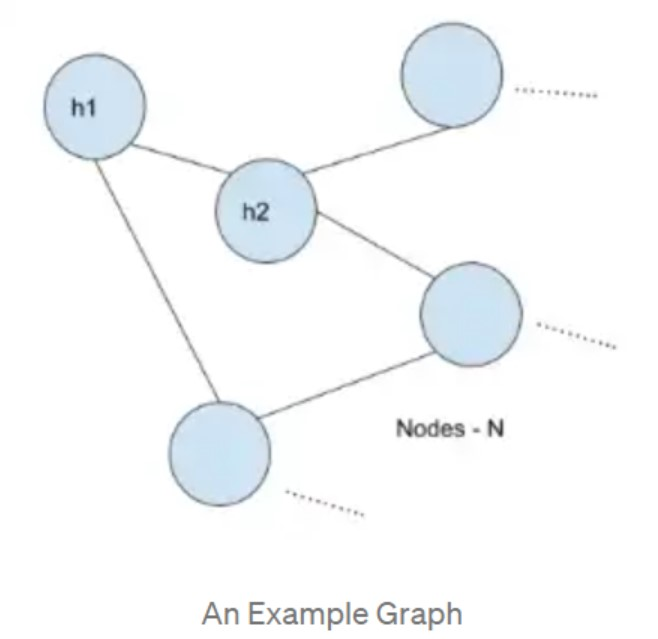
\includegraphics[width=4.79167in,height=4.63542in]{Picture/Fig1.jpg}
\end{center}

\subsubsection{Step 1 : Linear Transformation}
Step pertama dalam melakukan Graph Attentional Layer adalah dengan menerapkan transformasi linear. Weight matrix W ke vector dari node.

\subsubsection{Step 2 : Computation of Attention Coefficients}
Koefisien ini menentukan kepentingan dari node neighbornya. 

\begin{center}
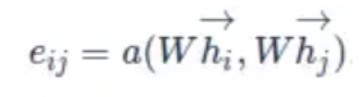
\includegraphics[width=2.54167in,height=0.69792in]{Picture/Fig2.jpg}    
\end{center}

dimana i,j adalah node tetangga atau neighbor, dan a adalah fungsi yang ditentukan dari persamaan berikut.

\begin{center}
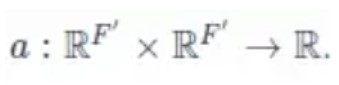
\includegraphics[width=2.63542in,height=0.51042in]{Picture/Fig3.jpg}
\end{center}

\begin{center}
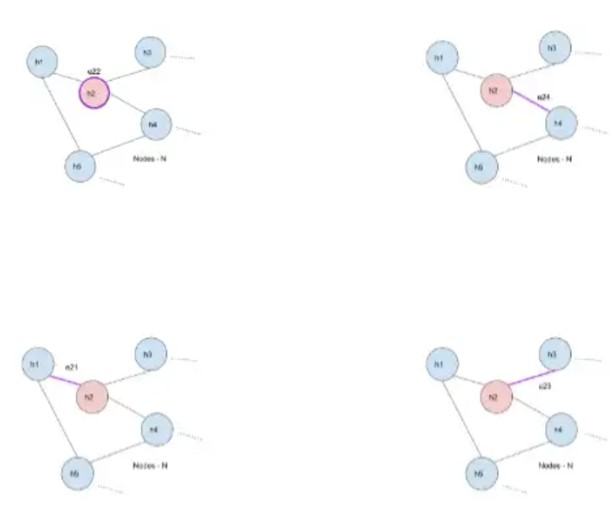
\includegraphics[width=4.52604in,height=3.37318in]{Picture/Fig4.jpg}
\end{center}

Gambar diatas merupakan visualisasi dari tiap step yang telah kita lakukan.

\subsubsection{Step 3 : Normalization of Attention Coefficients}
Karena struktur grafik yang bervariasi, node dapat memiliki jumlah neighbor atau tetangga yang berbeda. Untuk memiliki penskalaan umum di semua lingkungan, koefisien attention harus dinormalisasi.

\begin{center}
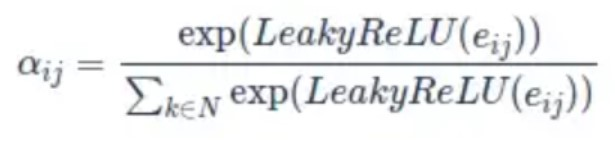
\includegraphics[width=4.63542in,height=0.97917in]{Picture/Fig5.jpg}
\end{center}

, dimana N adalah node tetangga dari node-i

\subsubsection{Step 4 : Computation of Final Output Features
}
Sekarang kami menghitung fitur node yang dipelajari. $\sigma$ adalah Transformasi Non-Linear.


Contoh dari arsitektural network,

\begin{center}
    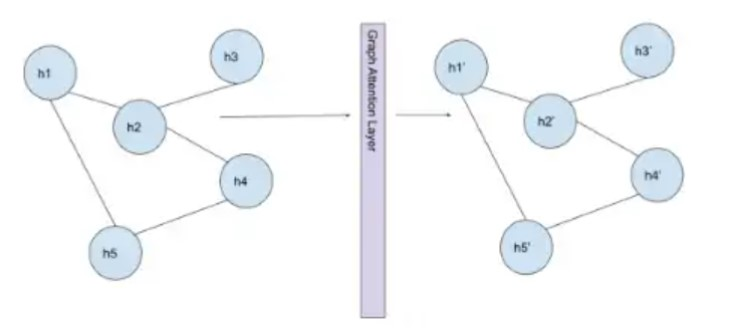
\includegraphics[width=5.11979in,height=2.18552in]{Picture/Fig6.jpg}
\end{center}

Dan formula untuk Learned Output Features,

\begin{center}
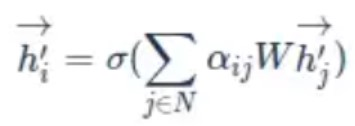
\includegraphics[width=2.72917in,height=0.85417in]{Picture/Fig7.jpg}
\end{center}

\subsubsection{Step 5 : Computation of Multiple Attention Mechanisms}
Untuk meningkatkan stabilitas proses pembelajaran, multi-head  attention digunakan. Kami menghitung beberapa jalur attentional yang berbeda dan akhirnya mengumpulkan semua representasi yang dipelajari.

\begin{center}
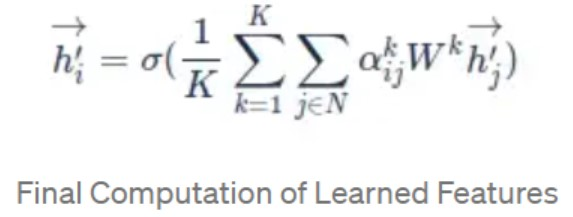
\includegraphics[width=3.85417in,height=1.54167in]{Picture/Fig8.jpg}
\end{center}

K menunjukkan jumlah jalur attention yang digunakan.

\begin{center}
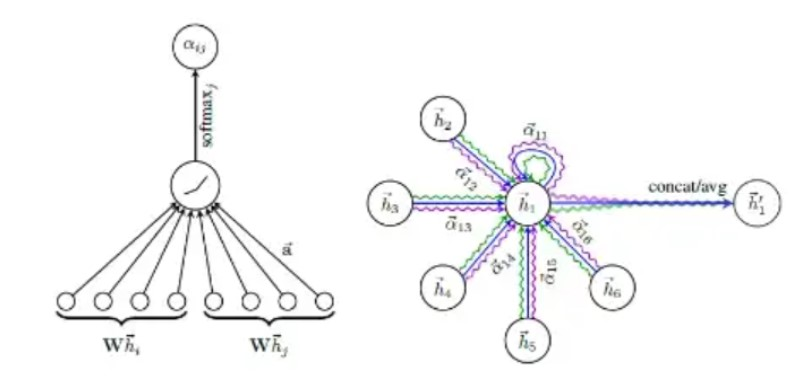
\includegraphics[width=5.25521in,height=2.51976in]{Picture/Fig9.jpg}
\end{center}

Gambar diatas merupakan tampilan keseluruhan pada semua operasi yang terlibat dalam pembaruan fitur node yang dipelajari.

\section{Result and Discussion}
Sebelumnya, telah disebutkan bahwa terdapat dua jenis konsep pada model GNN dengan arsitektur GAT, yaitu \textit{transductive} dan \textit{inductive}. Perbedaan antara kedua konsep itu adalah transductive menggunakan dataset yang memiliki satu grafik, seperti dataset Cora. Konsep utama dari jenis ini adalah tidak menggunakan informasi label dari node, melainkan menggunakan informasi seperti struktur dan fitur dari tiap node tersebut. Sedangkan jenis \textit{inductive} menggunakan grafik yang memiliki data terpisah antara \textit{validation, train}, dan \textit{test set}-nya.

Dalam penelitian ini, kami gunakan konsep \textit{transductive} dengan menggunakan dataset CORA. Dataset ini memiliki 2708 node, dimana setiap nodenya memiliki 1433 fitur. Dengan menggunakan dataset ini, kami terapkan pada permasalahan yang telah kami pilih, yaitu \textit{node classification}.

Kita gunakan arsitektur bawaan dari Graph Neural Network (GNN), yaitu Graph Attention Network (GAT) yang menerapkan mekanisme Attention. Konsep dari mekanisme ini adalah mempelajari kekuatan koneksi antar-tetangga node.

\subsection{Training Model GAT}
Dari eksperimen dari bentuk implementasi paper rujukan (Velickovic)\cite{cite26}, hasil dari pelatihan data pada model GAT yang kita dapatkan sebesar 0.8410 dengan loss sebesar 0.6626. Angka ini didapatkan dari pengulangan Epochs sebanyak 718 kali.

\begin{center}
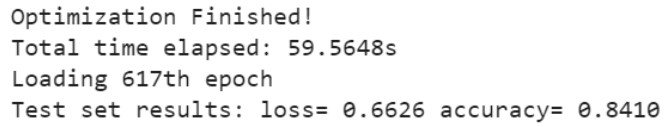
\includegraphics[width=4.64063in,height=0.97013in]{Picture/Fig11.jpg}
\end{center}

\subsection{Visualisasi Model}
Berdasarkan implementasi tersebut juga didapatkan visualisasi dari hasil eksperimen yang telah dilakukan.

\begin{center}
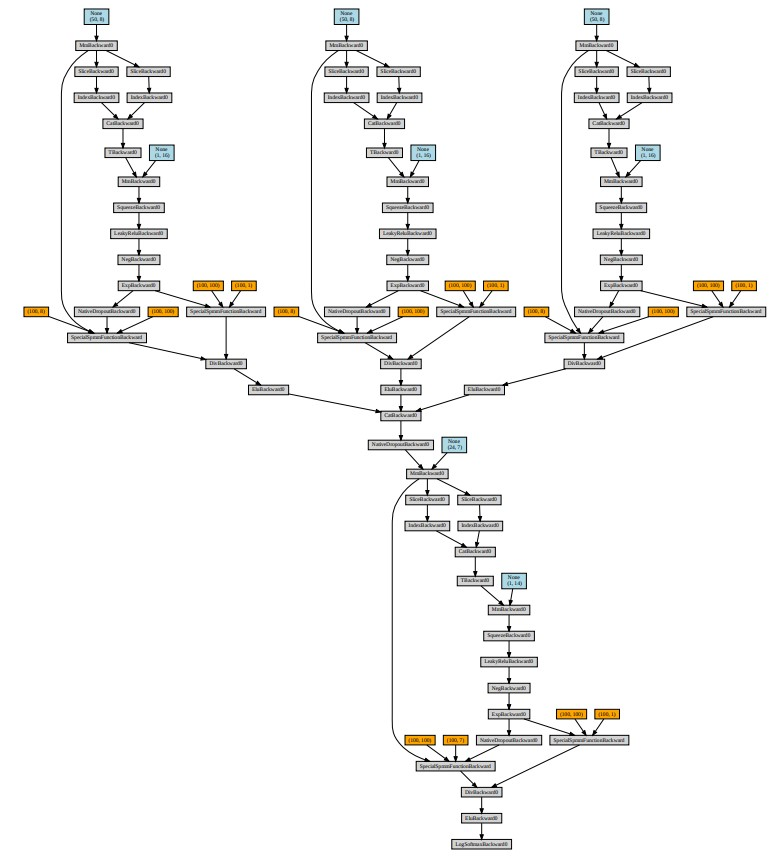
\includegraphics[width=4.71354in,height=5.22679in]{Picture/Fig10.jpg}
\end{center}

\subsection{Eksperimen antara GCN dan GAT}
Kami juga melakukan perbandingan antara dua model arsitektur dari GNN ini, yaitu GCN yang pernah diteliti oleh Kipf[16]. Pada penelitian ini, metode yang digunakan masih membutuhkan beberapa ketentuan, seperti \textit{eigendecompositions} dan operasi matriks tentang bobot dari node. 
Pada eksperimen dengan menggunakan arsitektur GCN ini, didapatkan hasil akurasinya sebesar 0.836 dengan train loss nya sebesar 0.7517.

\begin{center}
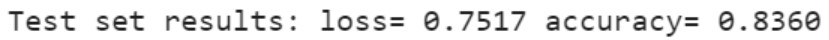
\includegraphics[width=6.15625in,height=0.35in]{Picture/Fig12.jpg}
\end{center}

\section{Conclusion}
Pada penelitian kali ini, kita menyelesaikan sebuah permasalahan \textit{node classification}, dimana kita diminta untuk melakukan pengenalan mengenai label dari node-node tetangganya. Tugas ini memprediksi atribut dari setiap node dalam grafik. Kita gunakan arsitektur berdasar mekanisme Attention untuk menyelesaikan tugas ini dari grafik yang ada pada dataset CORA. Dengan mekanisme ini, kita menghitung representasi tersembunyi dari setiap node dalam grafik, dengan memperhatikan tetangganya. Arsitektur ini disebut dengan Graph Attention Networks atau GATs. Lalu, dari arsitektur ini, kita juga lakukan perbandingan hasil yang didapatkan dari arsitektur yang memiliki kemiripan dengan GAT, yaitu GCN. Dari hasil eksperimen yang telah dilakukan, kita dapat melihat bahwa metode GAT memiliki akurasi yang lebih besar dibandingkan dengan metode GCN yaitu sebesar 84.1. Hal ini membuktikan bahwa metode GAT lebih baik digunakan untuk \textit{node classification} dibandingkan dengan metode GCN. 

\begin{center}
    \begin{tabular}{c|c}
    \hline
    \textbf{Metode} & \textbf{Akurasi}\\
    \hline
    {GCN} & {83.6} \\
    \hline
    \textbf{GAT} & \textbf{84.1}
    \end{tabular}
\end{center}

Dengan arsitektur GAT ini, terdapat solusi yang dapat diperoleh, seperti dapat memperluas metode untuk melakukan klasifikasi grafik pada klasifikasi node yang lebih relevan terhadap perspektif aplikasi. 

%Bibliography
\bibliographystyle{unsrt}  
\bibliography{references}  


\end{document}
